\subsubsection{Baza danych}
System korzysta z bazy danych SQLite3. W celu komunikacji z bazą danych z poziomu Erlanga wybrano erlang-sqlite3 (\url{https://github.com/alexeyr/erlang-sqlite3}). Persystowane są trzy rodzaje struktur: User, File oraz Action. Opisuje je rozdział 1.2 Struktury. Dla każdej z nich zdefiniowany jest odpowiedni moduł DAO: db\_users, db\_files oraz db\_actions. Wszystkie zostały przedstawione w poprzednich rozdziałach przy omawianiu modułów nadrzędnych.

Moduły DAO znajdują się w plikach:
\begin{itemize}
	\item storage/src/core/db\_files.erl
	\item storage/src/auth/db\_users.erl
	\item storage/src/core/db\_actions.erl
\end{itemize}

W przypadku chęci zmiany bazy danych, zmian wystarczy dokonać tylko w tych plikach (oraz dostarczyć odpowiedni sterownik). Jeden z prototypów działał z wykorzystaniem bazy MySQL.

\begin{figure}[!htbp]
	\centering
	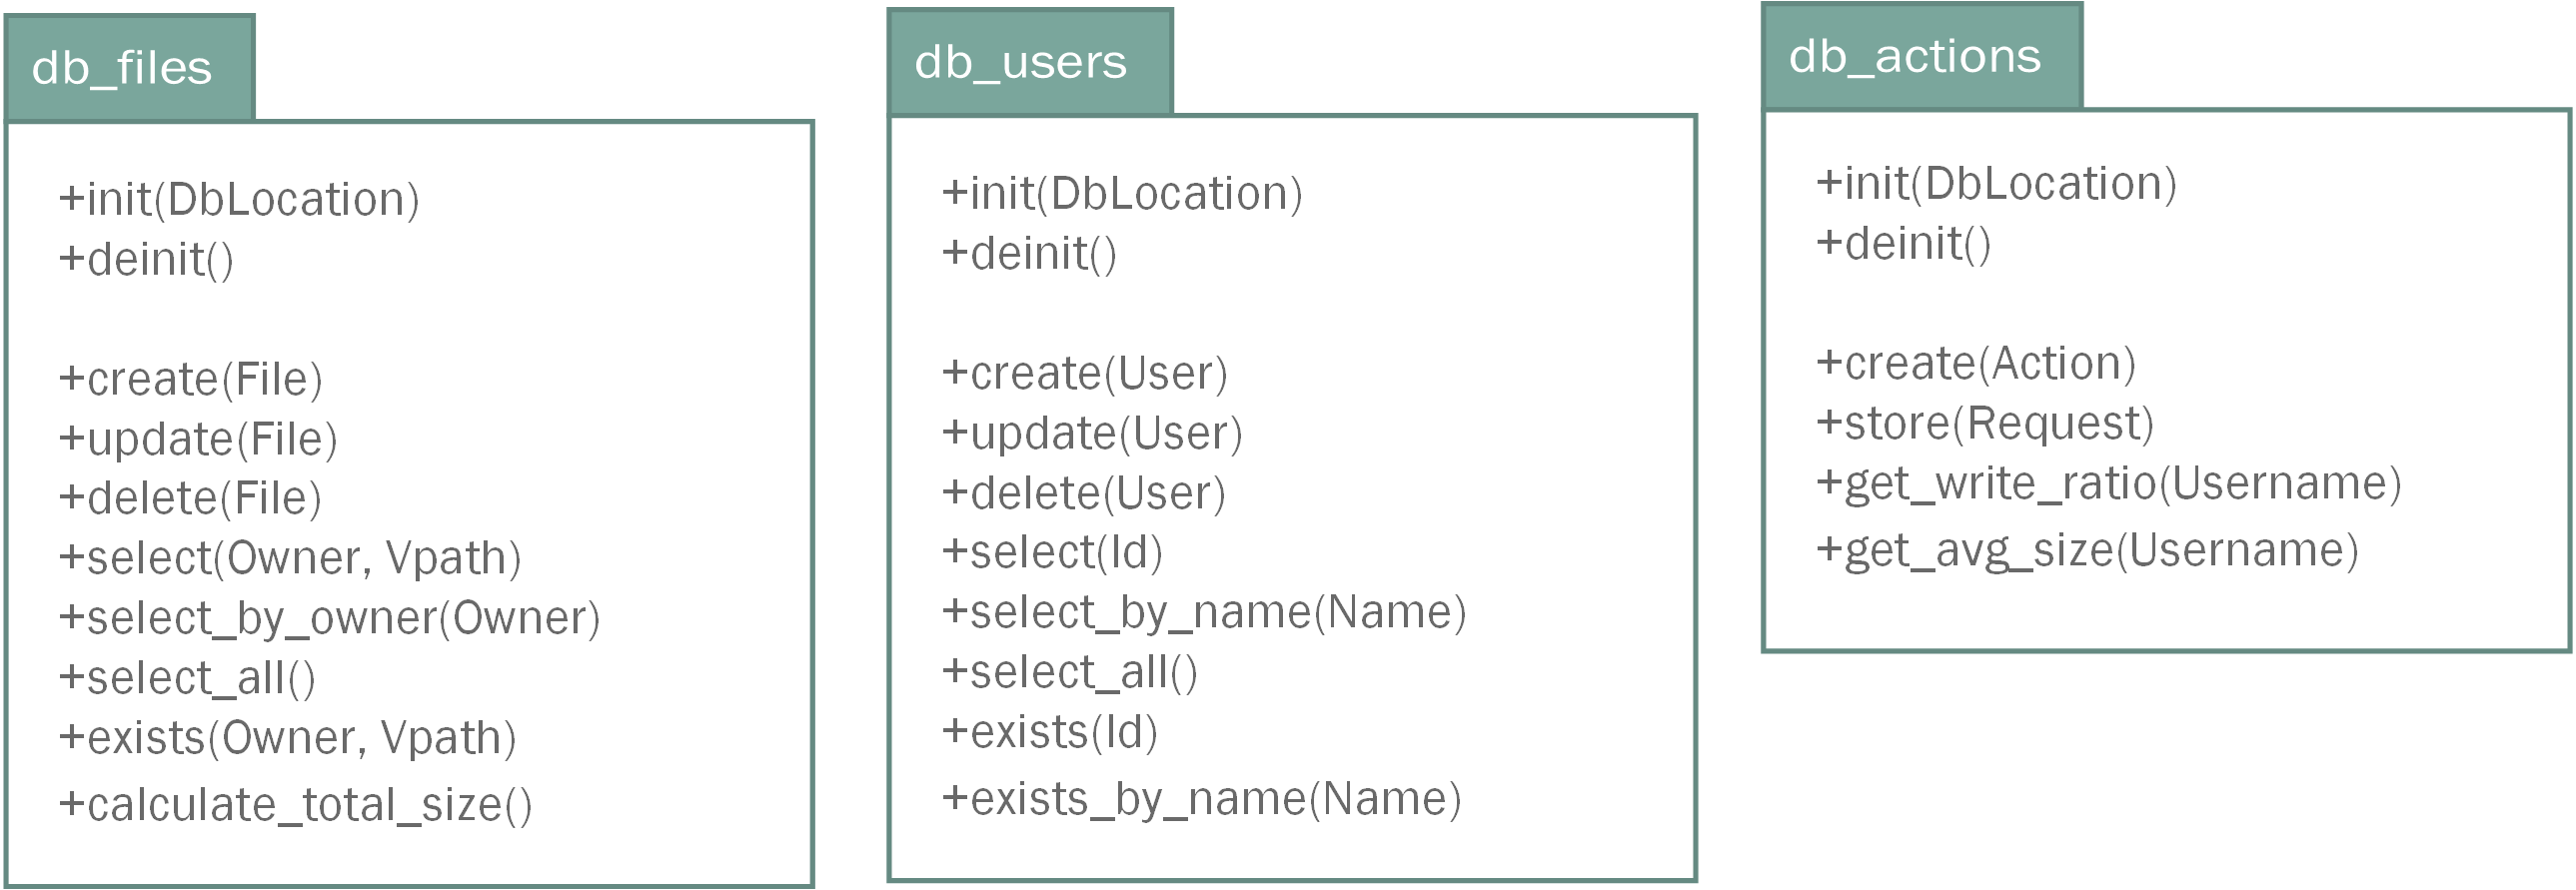
\includegraphics[width=0.9\textwidth]{db-modules}
	\caption[Struktura modułów DAO.]{Moduły DAO pozwalają zapisywać obiekty w bazie danych i wyszukiwać je na podstawie identyfikatora.}
	\label{fig:db-modules}
\end{figure}

\autoref{fig:db-erd} przedstawia diagram ERD bazy danych. Struktura tabel jest bardzo prosta jednak pozwala zrealizować wszystkie wymagania projektu.

Baza może pracować w standardowo, zapisując rekordy na dysku oraz w konfiguracji in-memory. Druga opcja przydatna może być w testach wydajnościowych. W celu jej aktywacji należy skompilować projekt z odpowiednią flagą. Więcej na temat kompilacji mówi rozdział 3.3 Kompilacja.

\begin{figure}[!htbp]
	\centering
	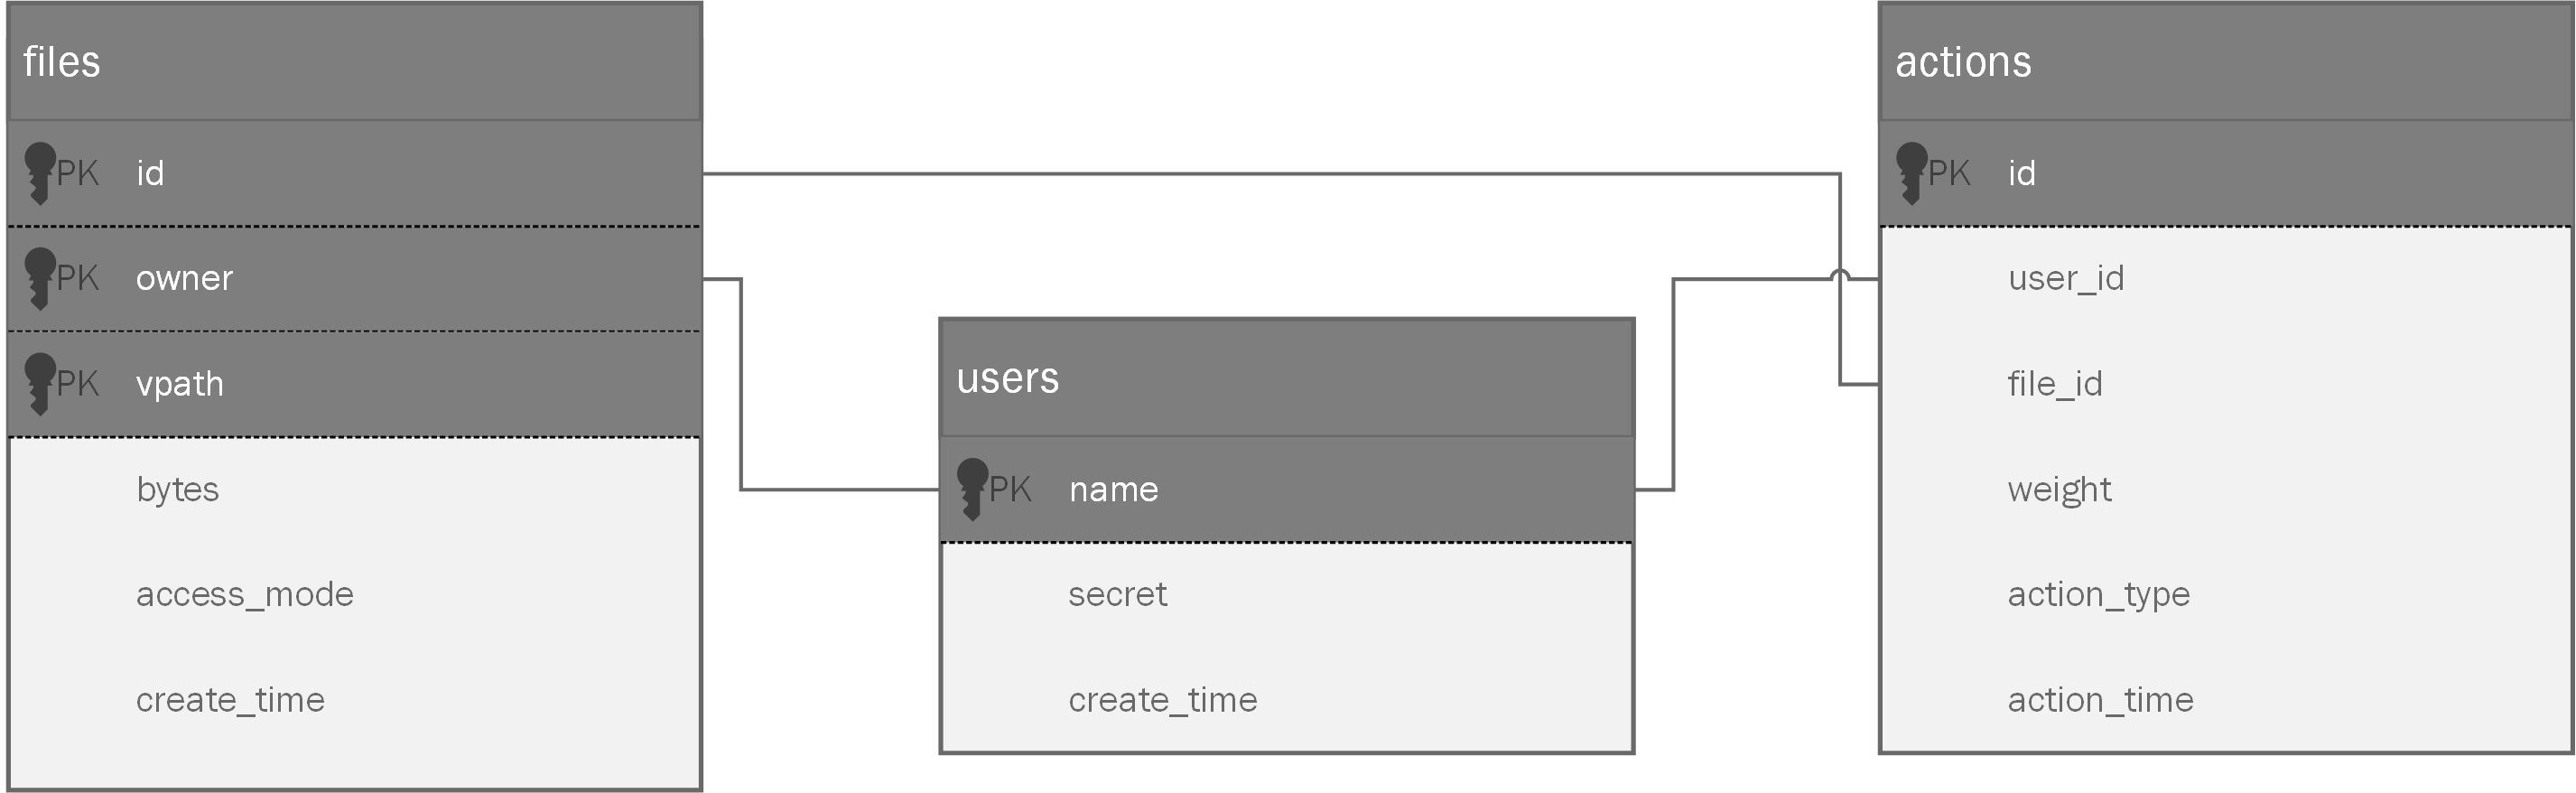
\includegraphics[width=0.9\textwidth]{db-erd}
	\caption{Baza danych - diagram ERD}
	\label{fig:db-erd}
\end{figure}